\documentclass[git]{deltares_manual_dfastbe}

\usepackage{tikz}
\usepackage[pipeTables=true]{markdown}

%------------------------------------------------------------------------------
\newcommand{\dfastbe}{\textrm{D-FAST~Bank~Erosion}\xspace}
\newcommand{\dfbe}{\textrm{D-FAST~BE}\xspace}
\newcommand{\dflowfm}{\textrm{D-Flow~FM}\xspace}

% Distribution version: written by the build (CI / BuildScripts) from pyproject.toml,
% which commitizen bumps during the release workflow. Fallback keeps local compiles working.
\providecommand{\dfbeversion}{0.0.0}
\InputIfFileExists{version.tex}{}{}

\hypersetup
{
    pdfauthor   = {Deltares},
    pdftitle    = {\dfastbe},
    pdfkeywords = {Technical Reference \dfastbe}
}

\begin{document}
\pagestyle{empty}
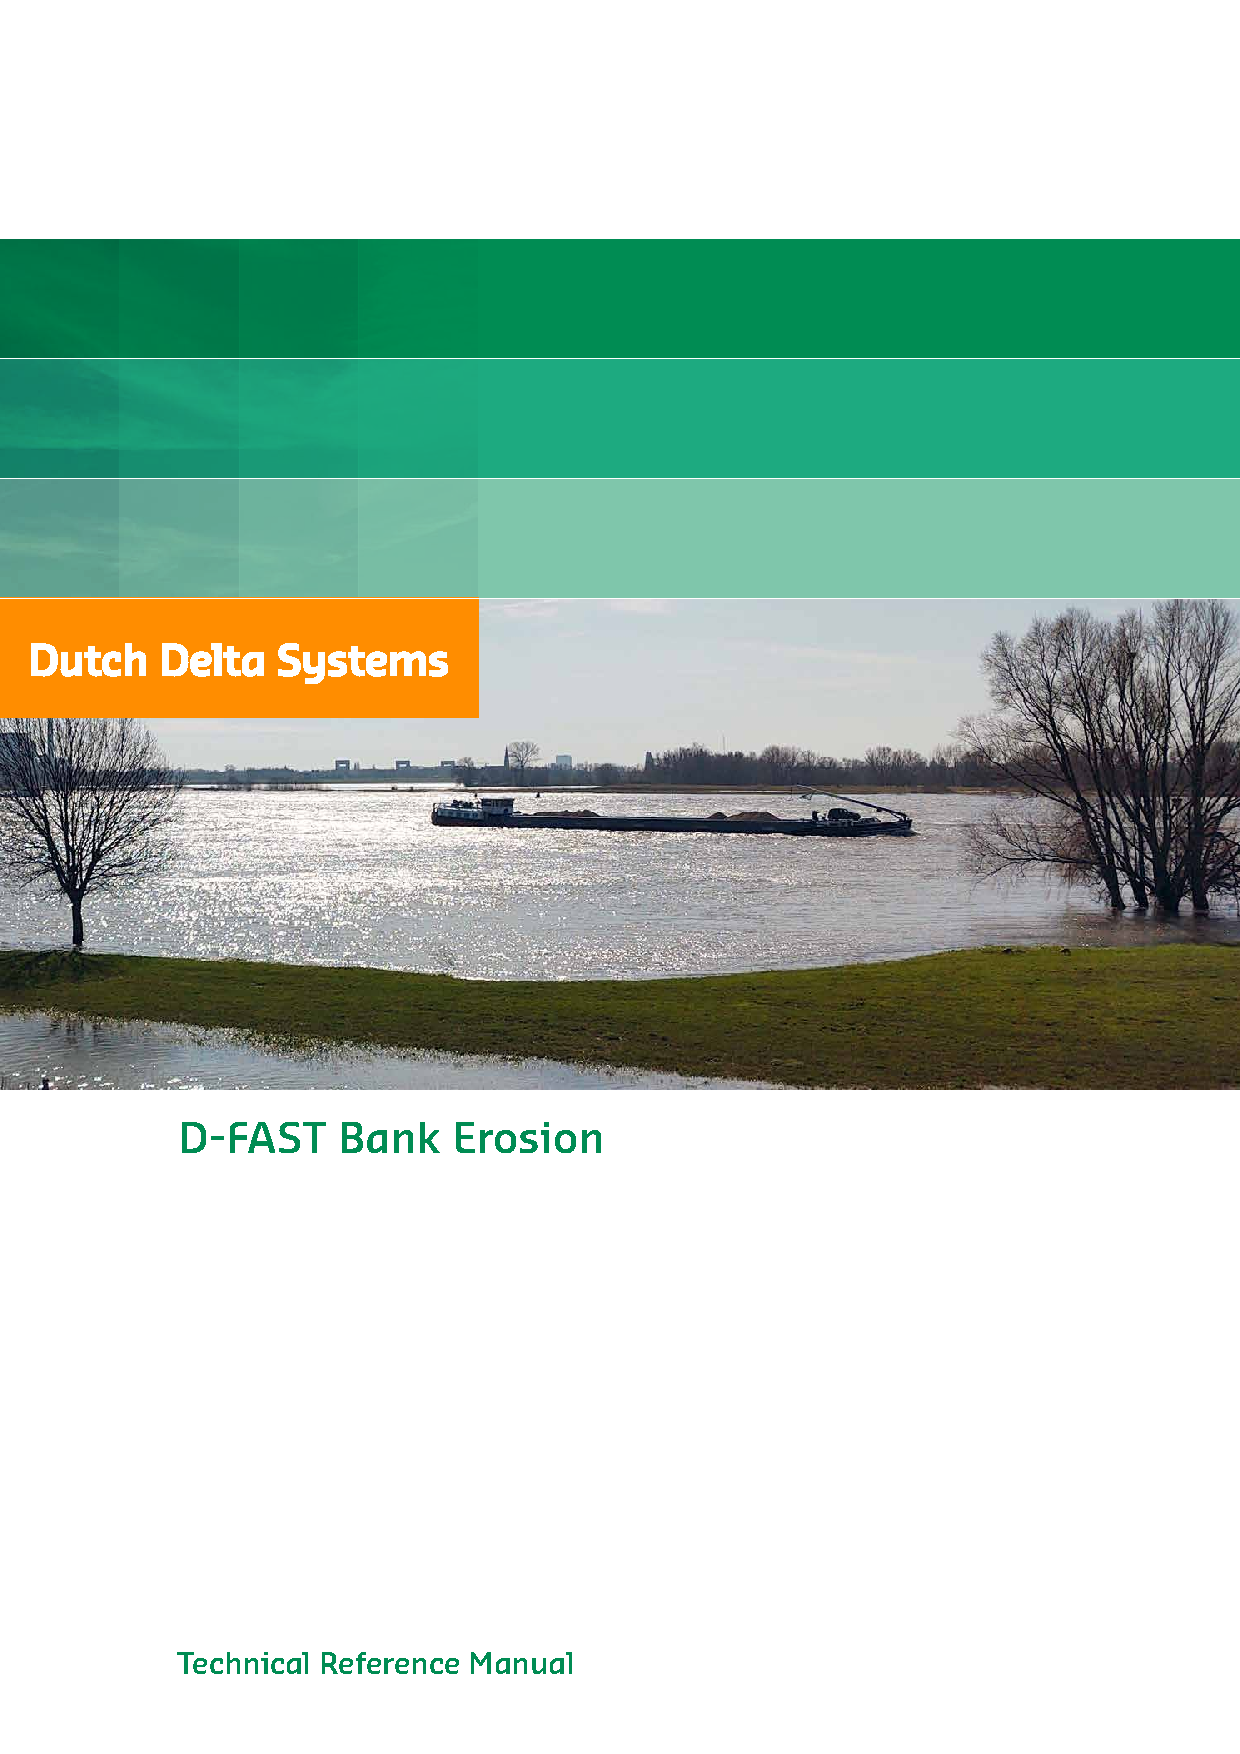
\includepdf[pages=1, offset=72 -70]{cover/D-FAST-omslag-D-FAST Bank Erosion-TRN.pdf} % links-rechts past precies
\cleardoublepage
\title{D-FAST\\ Bank Erosion}
\subtitle{}
\manualtype{Technical Reference Manual and Test Report}
\distribution{Released for: \newline \phantom{M} \dfbe version \dfbeversion\ or higher}
\version{\the\year.\ifnum\month<10 0\fi\the\month}

\author{ }

\setgitdirectory{../.git}
\deltarestitle
%
\include{chapters/intro_tech}

\include{chapters/requirements}
\include{chapters/code_structure}
\chapter{Software maintenance}

\section{Coding guidelines}

This program has been implemented following the Python PEP 8 style guide and targets Python 3.11
or newer; the exact supported range is declared in \keyw{pyproject.toml}.
The code has been documented using standard Python docstrings and type hinting.

Code quality is enforced automatically through a \keyw{pre-commit} configuration
(\keyw{.pre-commit-config.yaml}) that runs locally on the developer's machine before each commit.
The key checks include (see \keyw{.pre-commit-config.yaml} for the complete set):

\begin{itemize}
\item \emph{Black} for code formatting, with a line length of 88 characters that is shared with
\keyw{isort} and \keyw{flake8} (the \keyw{[tool.black]}, \keyw{[tool.isort]} and \keyw{[tool.flake8]}
sections of \keyw{pyproject.toml});
\item \emph{isort} for import ordering;
\item \emph{flake8} (with the \keyw{flake8-bugbear} and \keyw{flake8-docstrings} plugins) for linting
and PEP~257 docstring conventions; new docstrings follow the Google style;
\item \emph{bandit}, \emph{gitleaks}, \emph{detect-secrets}, \emph{trufflehog}, \emph{checkov} and
\emph{detect-private-key} for security and secret scanning;
\item \emph{beautysh} and \emph{shell-lint} for the shell and \keyw{.bat} build scripts;
\item \emph{commitizen} together with a set of commit-message hooks (imperative mood, capitalisation,
length and punctuation of the summary, blank second line) to enforce the Conventional Commits format;
\emph{commitizen} also drives version bumping and change-log generation (the \keyw{[tool.commitizen]}
section, \keyw{update\_changelog\_on\_bump});
\item a set of file-hygiene hooks (trailing whitespace, end-of-file, mixed line endings, large-file
guard, merge-conflict markers, JSON/YAML/TOML validation) and a \keyw{no-commit-to-branch} guard that
blocks direct commits to \keyw{main};
\item \emph{pytest} (unit, doctest and notebook runs) executed as local hooks, excluding the
end-to-end and binary tests.
\end{itemize}

The formatting and linting settings are defined in \keyw{pyproject.toml} (the \keyw{[tool.black]},
\keyw{[tool.isort]} and \keyw{[tool.flake8]} sections).
To run the full set of checks manually, install \keyw{pre-commit} and execute:

\begin{Verbatim}
    > pre-commit run --all-files
\end{Verbatim}

The \keyw{pre-commit} hooks are not run by continuous integration; they are intended to be installed
and run on the developer's machine. Continuous integration (the \keyw{testing.yml} GitHub Actions
workflow) instead runs the \keyw{pytest} test suite (excluding the binary tests) across a matrix of
Python 3.11--3.13 on Linux and Windows using Poetry, and uploads the coverage results to Codecov.
A minimum overall line-coverage threshold of 61\% is enforced; see \autoref{Chp:TestPlan} for details
of the test suite.

\section{Version control}

GitHub is currently used for software version control.
The repository is located at \url{https://github.com/Deltares/D-FAST_Bank_Erosion}.
Since \dfastbe builds on WAQBANK, the initial release of the new Python product is labeled as version 2.0.0.
%We may switch to GitLab in line with \href{http://publicaties.minienm.nl/documenten/rijkswaterstaat-informatievoorziening-aansluitvoorwaarden-riva-2017}{RIVA (2020)}.

\section{Automated building of code}

The standalone Windows executable is built locally with the \emph{Nuitka} compiler, driven by the
scripts in \keyw{BuildScripts} (\keyw{BuildDfastbe.bat}, or \keyw{BuildDfastbe\_no\_command\_window.bat}
for a build without a console window). The script reads the version number from \keyw{poetry version}
and invokes Nuitka roughly as follows:

\begin{Verbatim}
python -m nuitka --standalone --mingw64 --enable-plugin=pyside6 --enable-plugin=anti-bloat
    --python-flag=no_site --python-flag=no_asserts --python-flag=no_docstrings
    --include-package=numpy --include-package=pyproj --include-module=shapely
    --include-package=matplotlib --include-package=netCDF4 --include-package=cftime
    --include-module=geopandas --include-package=pandas --include-package=pytz
    --include-package-data=geopandas.datasets --include-module=fiona
    --include-data-files=src/dfastbe/io/log_data/messages.UK.ini=dfastbe/io/log_data/messages.UK.ini
    --file-reference-choice=runtime src/dfastbe
\end{Verbatim}

Unfortunately, this doesn't automatically build a binary that works out of the box.
The following adjustments depend on the exact combination of Nuitka and package versions used, so they will need to be revisited when updating the software.
A number of environmental settings (together with an explicit \keyw{pyproj} data-directory setup) had
to be added to \keyw{\_\_main\_\_} so that the standalone executable locates its bundled data
directories at runtime; these are settings that the Nuitka compiler did not resolve automatically.

\begin{Verbatim}
import os
from pathlib import Path

import matplotlib

matplotlib.use("Qt5Agg")

is_nuitka = "__compiled__" in globals()
if is_nuitka:
    """Needed for Nuitka compilation"""

    root = str(Path(__file__).parent)
    os.environ["GDAL_DATA"] = root + os.sep + "gdal"
    os.environ["PROJ_LIB"] = root + os.sep + "proj"
    os.environ["MATPLOTLIBDATA"] = root + os.sep + "matplotlib" + os.sep + "mpl-data"
    os.environ["TCL_LIBRARY"] = root + os.sep + "lib" + os.sep + "tcl8.6"
    proj_lib_dirs = os.environ.get("PROJ_LIB", "")
    import pyproj.datadir

    pyproj.datadir.set_data_dir(root + os.sep + "proj")
    import pyproj
\end{Verbatim}

If these environment settings are not applied, the standalone executable fails to locate its bundled
data directories at runtime, producing errors such as a missing PROJ, matplotlib or Tcl/Tk data
directory.

The Nuitka options above already bundle the required packages together with the data files that the
tool needs at runtime: the language files \keyw{messages.NL.ini} and \keyw{messages.UK.ini}, the GUI
icons, the licence file and the three PDF manuals.

A few shared libraries that Nuitka places in separate \keyw{*.libs} folders still have to be moved
next to the packages that load them. This is handled automatically by \keyw{BuildScripts/Move\_Libs.bat},
which moves the contents of \keyw{pyproj.libs}, \keyw{matplotlib.libs} and \keyw{fiona.libs} into the
corresponding \keyw{pyproj}, \keyw{matplotlib} and \keyw{fiona} folders of the distribution:

\begin{Verbatim}
move dfastbe.dist\pyproj.libs\*     dfastbe.dist\pyproj
move dfastbe.dist\matplotlib.libs\* dfastbe.dist\matplotlib
move dfastbe.dist\fiona.libs\*      dfastbe.dist\fiona
\end{Verbatim}

Finally, \keyw{BuildScripts/Collect\_Examples.bat} copies the example data sets into the distribution.
At runtime, the environment settings shown above point \keyw{pyproj}, GDAL, PROJ, matplotlib and
Tcl/Tk to the corresponding data directories inside the bundled distribution, so no further manual
copying of data directories or DLLs is required.

\section{Listing of external modules}

The runtime and development dependencies of \dfastbe --- including the supported Python version range
and the pinned version constraints --- are declared in \keyw{pyproject.toml}.
Refer to that file (and the accompanying lock file) for the authoritative, up-to-date list of
external modules rather than a static snapshot that quickly becomes outdated.

The main runtime dependencies are \keyw{numpy}, \keyw{pandas}, \keyw{geopandas}, \keyw{shapely},
\keyw{netCDF4}, \keyw{matplotlib}, \keyw{Pillow}, \keyw{pyside6} and \keyw{dfastio}.
Additional development, documentation and binary-build dependencies are grouped under the
\keyw{[dependency-groups]} section of \keyw{pyproject.toml}.

\section{Automated testing of code}

See \autoref{Chp:TestPlan} and \autoref{Chp:TestReport}.

\section{Automated generation of documentation}

The documentation has been written in a combination of LaTeX and markdown files which are maintained in the GitHub repository alongside the source code.
The PDF version of the user manual and this technical reference manual are generated automatically as part of the daily cycle of building all manuals on the Deltares TeamCity server.
\chapter{Test Plan} \label{Chp:TestPlan}

The results of the software is verified by means of

\begin{itemize}
\item Unit testing at the level of functions, such as reading and writing of files, and basic testing of the algorithms.
A large part of the code base --- in particular the \keyw{io}, \keyw{bank\_lines} and \keyw{bank\_erosion} sub-packages --- is covered by unit tests, and a minimum overall line-coverage threshold (currently 61\%) is enforced.
These tests are carried out by means of the \keyw{pytest} framework.
\item Regression tests have been configured to verify that the results of the batch mode remain
unchanged under further code developments.
\end{itemize}

For the verification of \dfastbe three sets of input files for the Meuse River have been used:

\begin{enumerate}
\item One set of WAQUA result files converted using \keyw{sim2ugrid.m} to \dflowfm like netCDF files.
\item One set of \dflowfm result files of simulations using the same curvilinear mesh as was used in WAQUA.
\item One set of \dflowfm result files of simulations using a new unstructured mesh.
\end{enumerate}

Each configuration gives slightly different results; for further regression testing in particular the first and last one will be used.
For the automated testing, unit tests and regression tests based on known input/output combinations will be used.
These tests will be executed on the original Python code (i.e. in source code form) and to the degree possible on the compiled binaries as well.

\section{Acceptance testing}

In \autoref{Sec:FuncReq} the 10 functional requirements were listed.
They are repeated below and for every requirement it is indicated how it is tested.

\begin{enumerate}
\item The results of \dfastbe must match those of WAQBANK given the same input data.
This is tested by means of a number of comparison studies, and subsequently tested using regression tests.

\item Users must be able to run this program in batch mode from the command line.
This has been implemented as run modes \keyw{-{}-mode banklines} and \keyw{-{}-mode bankerosion}.
The proper functioning of these options is tested by means of regression testing.

\item Users must be able to run the analysis based on \dflowfm results.
This is tested by means of regression testing using result files of \dflowfm version 1.2.105.67088.

\item Users must be able to provide all data via an input file, similar to the ini-file like file of WAQBANK.
This testing is included in the regression testing of the batch mode, and is also covered by the
automated GUI tests.

\item The input files must be consistent with those of WAQBANK, or aligned with open standards or the \dflowfm modeling system.
The \dfastbe configuration file is identical to the WAQBANK definition file except for the fact that the new file contains three sections \keyw{[General]}, \keyw{[Detect]} and \keyw{[Erosion]} to give a bit more context for the purpose of each keyword.
\dfastbe accepts old WAQBANK input files, but writes the data in the new format.
The format of the other input files is not adjusted, but for line geometries \dfastbe also accepts shape files besides the original \file{.xyc} files.
There are unit and integration tests addressing the reading of the input files.

\item The output files must be consistent with those of WAQBANK, or aligned with open standards or the \dflowfm modeling system.
The ASCII files containing the bank erosion volumes are identical to those of WAQBANK.
The shifted bank lines are exported as Shape files instead of \file{.xyc} files to align with common GIS standards.
The figures are now saved as \file{.png} files instead of MATLAB specific \file{.fig} files.
There are unit and integration tests addressing the writing of the output files.

\item The should read relevant data directly from \dflowfm map-files similarly to WAQBANK reading data directly from SIMONA and Delft3D 4 result files.
All quantities previously read from the SIMONA SDS-files and Delft3D-FLOW trim-files is now read from the \dflowfm map.nc files.

\item A simple graphical user interface could support users in process of creating the input file.
The graphical user interface that you get by running \dfastbe in default mode or by explicitly specifying \keyw{-{}-mode gui} has been tested manually as described in \autoref{Sec:GuiTests}.

\item It would be nice if the software would be more generally applicable than just the Dutch rivers.
The code does not include specific knowledge of the Dutch rivers except for the fact that some of the rules of thumb have been derived using Dutch river data.
The original WAQBANK code was already applied to foreign rivers such as the Danube.
No special testing carried out for this requirement.

\item It would be nice if the software would be able to run besides English also in Dutch.
All texts shown by \dfastbe are read from a language configuration file.
An English and a Dutch version of that configuration file are provided.
A most system tests are carried out using the default English configuration, but one test is carried out using the Dutch configuration.
\end{enumerate}

\section{System testing}

The whole system is tested via the command line (entry via \keyw{\_\_main\_\_}) and via Python calls to the \keyw{run()} method of the \keyw{Runner} class in the \keyw{runner} module.
These tests are repeated for the standalone compiled \dfastbe executable.
For the system testing a limited number of regression tests are carried out comparing the latest results against previously accepted results.

The graphical user interface is covered by automated tests that use the \keyw{pytest-qt} plugin (the
\file{tests/test\_gui} suite). In addition, a protocol for manual user-interface tests has been
defined; these manual tests are described in the following section.

\subsection{Manual testing of the user interface} \label{Sec:GuiTests}

\subsubsection{Test 1: starting blank}
\subsubsection{Test 2: save default configuration file}
\subsubsection{Test 3: modify general settings}
\subsubsection{Test 4: modify detection settings}
\subsubsection{Test 5: modify erosion settings}
\subsubsection{Test 6: save modified configuration file}
\subsubsection{Test 7: load default configuration file}
\subsubsection{Test 8: load modified configuration file}
\subsubsection{Test 9: run detection analysis}
\subsubsection{Test 10: run erosion analysis}
\subsubsection{Test 11: view manual and about Windows}

\section{Integration testing}

The \keyw{bank\_lines} and \keyw{bank\_erosion} sub-packages build on the functionality of the \keyw{io} and \keyw{plotting} modules to provide the bank line detection and erosion analysis workflows.
These workflows are driven through the \keyw{Runner} class in the \keyw{runner} module and are tested at this level via integration and regression tests, while the supporting routines are tested as part of the unit testing.

\section{Unit testing}

The automated test suite lives under \file{tests} and is organised per sub-package; it currently
comprises about 275 tests. The main groups are:

\begin{itemize}
\item \file{tests/test\_io} --- configuration parsing, file reading and writing, and logging
(\file{test\_io.py}, \file{test\_logging.py});
\item \file{tests/test\_bank\_lines} --- the bank line detection workflow and its data models;
\item \file{tests/test\_erosion} --- the bank erosion workflow, data models, the erosion calculator
and the mesh processor;
\item \file{tests/test\_gui} --- the graphical user interface (see below);
\item \file{tests/test\_cli\_main.py} --- the command-line entry point.
\end{itemize}

Since the \keyw{io}, \keyw{bank\_lines}, \keyw{bank\_erosion} and \keyw{plotting} packages only depend
on third-party modules, they are well suited for unit testing and are covered in detail.

\subsection{Graphical user interface testing}

The \keyw{gui} package interacts with the graphical user interface by reading from and writing to the
state of the controls. These routines are tested automatically with the \keyw{pytest-qt} plugin (the
\file{tests/test\_gui} suite, about 140 tests), which drives the Qt widgets without requiring manual
interaction. The suite covers the configuration loader and exporter, dialog creation, the GUI
utilities, and each settings tab (General, Detection, Erosion, Bank Parameters and Shipping
Parameters). The manual user-interface protocol described above complements these automated tests.

The \keyw{pytest-qt} plugin lets the tests drive the real \keyw{PySide6} widgets in-process, without a
human operator. It provides two key pytest fixtures:

\begin{itemize}
\item \keyw{qapp} --- a single shared \keyw{QApplication} for the test session. On a headless machine
(for example the Linux continuous-integration runner without a display) it is started with the Qt
\keyw{offscreen} platform, so the widgets are created and exercised entirely in memory and no window
ever appears on screen.
\item \keyw{qtbot} --- a helper that registers a widget with the test (\keyw{qtbot.addWidget}),
simulates user interaction such as mouse clicks (\keyw{qtbot.mouseClick}), and waits for the
application to process events or emit signals (\keyw{qtbot.wait}, \keyw{qtbot.waitSignal}).
\end{itemize}

A typical GUI test follows the same pattern a user would: it builds the relevant part of the interface
through the project's own fixtures (for example \keyw{setup\_gui}, which instantiates the full
\keyw{GUI} with all tabs, or the per-component \keyw{setup\_menubar} and \keyw{setup\_button\_bar}
fixtures in \file{tests/test\_gui/conftest.py}), then puts the controls into a known state by setting
their values directly (\keyw{setText} on a line edit, \keyw{setChecked} on a check box,
\keyw{setCurrentText} on a drop-down) or by triggering an action with \keyw{qtbot.mouseClick}, and
finally asserts on the result. The two main things asserted are: (i) that the widgets are created and
laid out as expected (located with \keyw{findChildren}), and (ii) that the data round-trips correctly
--- loading a configuration file populates the controls with the right values, and exporting the
controls reproduces the original configuration. Because everything runs in memory, these tests are
fast and require no manual clicking.

\subsection{Binary testing}

The standalone executable is verified by a separate set of tests marked with the \keyw{binaries}
marker (\file{tests/test\_binaries}). These run the compiled \dfastbe binary and are executed on
TeamCity; they are excluded from the GitHub Actions run with \keyw{-m "not binaries"}.

\section{Automated testing}

The Python code is tested automatically by a GitHub Actions workflow (\keyw{testing.yml}) that runs
the \keyw{pytest} suite on every push across a matrix of Python 3.11--3.13 on Linux and Windows and
uploads the coverage to Codecov. The binary tests are excluded there (\keyw{-m "not binaries"}); the
standalone binaries are built with the \keyw{BuildScripts} and tested on TeamCity.

For all automated unit and regression tests the pytest framework is used. After installing the
development dependencies with Poetry, the suite is run with:

\begin{Verbatim}
    > poetry run pytest
\end{Verbatim}

\subsection{Test coverage}

Coverage is measured with \keyw{pytest-cov}. A minimum overall line coverage of 61\% is enforced
(\keyw{fail\_under} in \keyw{pyproject.toml}); the run fails below that threshold. A recent run reports
an overall coverage of about 90\%. The line coverage of the main source packages is summarised below.

\begin{tabular}{l|r}
Package & Line coverage \\ \hline
\keyw{io} & 91\% \\
\keyw{bank\_lines} & 94\% \\
\keyw{bank\_erosion} & 88\% \\
\keyw{gui} & 72\% \\
module-level files (\keyw{runner}, \keyw{plotting}, \keyw{utils}, \dots) & 89\% \\
\end{tabular}

%-------------------------------
\chapter{Test Report} \label{Chp:TestReport}

The test plan describes manual tests (the graphical user interface tests as part of the system testing) and automated testing (unit and regression testing).

\section{Manual tests}

This section summarizes the results of the manual testing of the graphical user interface.

\begin{tabular}{ll|l}
Test & Description & Success / Comments \\ \hline
1 & starting blank & OK \\
2 & save default configuration file & OK \\
3 & modify general settings & OK \\
4 & modify detection settings & OK \\
5 & modify erosion settings & OK \\
6 & save modified configuration file & OK \\
7 & load default configuration file & OK \\
8 & load modified configuration file & OK \\
9 & run detection analysis & OK \\
10 & run erosion analysis & OK \\
11 & view manual and about Windows & OK \\
\end{tabular}

\section{Automated tests}

The automated regression and unit tests are run with \keyw{pytest} and \keyw{pytest-cov}. The full
per-file coverage report of a recent run (with the binary tests deselected) is included below. The
per-line "Missing" column of the original report is omitted here for brevity.

\begin{Verbatim}[fontsize=\tiny]
================================== test session starts ==================================
platform win32 -- Python 3.11.12, pytest-9.0.3, pluggy-1.5.0
configfile: pyproject.toml
plugins: cov-7.0.0, qt-4.4.0
collected 275 items / 6 deselected / 269 selected

---------- coverage: platform win32, python 3.11.12-final-0 ----------
Name                                                   Stmts   Miss  Cover
--------------------------------------------------------------------------
src\dfastbe\__init__.py                                    7      2    71%
src\dfastbe\__main__.py                                   47     12    74%
src\dfastbe\bank_erosion\__init__.py                       0      0   100%
src\dfastbe\bank_erosion\bank_erosion.py                 258      4    98%
src\dfastbe\bank_erosion\data_models\__init__.py           0      0   100%
src\dfastbe\bank_erosion\data_models\calculation.py      223     15    93%
src\dfastbe\bank_erosion\data_models\inputs.py           204     11    95%
src\dfastbe\bank_erosion\debugger.py                      39      0   100%
src\dfastbe\bank_erosion\erosion_calculator.py            77      0   100%
src\dfastbe\bank_erosion\mesh\__init__.py                  0      0   100%
src\dfastbe\bank_erosion\mesh\data_models.py             146     65    55%
src\dfastbe\bank_erosion\mesh\processor.py               294     85    71%
src\dfastbe\bank_erosion\plotter.py                      282      3    99%
src\dfastbe\bank_erosion\utils.py                        283     31    89%
src\dfastbe\bank_lines\__init__.py                         0      0   100%
src\dfastbe\bank_lines\bank_lines.py                     133      1    99%
src\dfastbe\bank_lines\data_models.py                     67      0   100%
src\dfastbe\bank_lines\plotter.py                         62      0   100%
src\dfastbe\bank_lines\utils.py                          144     22    85%
src\dfastbe\base_calculator.py                            17      0   100%
src\dfastbe\gui\__init__.py                                0      0   100%
src\dfastbe\gui\application.py                            89     12    87%
src\dfastbe\gui\base.py                                  137     56    59%
src\dfastbe\gui\configs.py                               344     48    86%
src\dfastbe\gui\state_management.py                       14      1    93%
src\dfastbe\gui\tabs\analysis_runner.py                   48     28    42%
src\dfastbe\gui\tabs\bank.py                              51      0   100%
src\dfastbe\gui\tabs\detection.py                         25      0   100%
src\dfastbe\gui\tabs\discharge_levels.py                  41     29    29%
src\dfastbe\gui\tabs\erosion.py                           48      0   100%
src\dfastbe\gui\tabs\general.py                           82      0   100%
src\dfastbe\gui\tabs\main_components.py                  101     30    70%
src\dfastbe\gui\tabs\shipping.py                          20      0   100%
src\dfastbe\gui\utils.py                                 284    151    47%
src\dfastbe\io\__init__.py                                 0      0   100%
src\dfastbe\io\config.py                                 475     57    88%
src\dfastbe\io\data_models.py                            274     11    96%
src\dfastbe\io\file_utils.py                              20      0   100%
src\dfastbe\io\logger.py                                  75      6    92%
src\dfastbe\plotting.py                                  114      9    92%
src\dfastbe\runner.py                                     40      3    92%
src\dfastbe\utils.py                                      68      6    91%
--------------------------------------------------------------------------
TOTAL                                                   7198    706    90%

Required test coverage of 61.0% reached. Total coverage: 90.19%
====================== 269 passed, 6 deselected in 135.42s (0:02:15) ======================
\end{Verbatim}


\appendix
\include{chapters/file_formats}

\pagestyle{empty}
\cleardoublepage
\mbox{}
\includepdf[pages=2, offset=-72 -70]{cover/D-FAST-omslag-D-FAST Bank Erosion-TRN.pdf} % links-rechts past precies
\end{document}
